\subsection{Subsystem $<$Views$>$}

\subsubsection{Detailed Design Diagram}
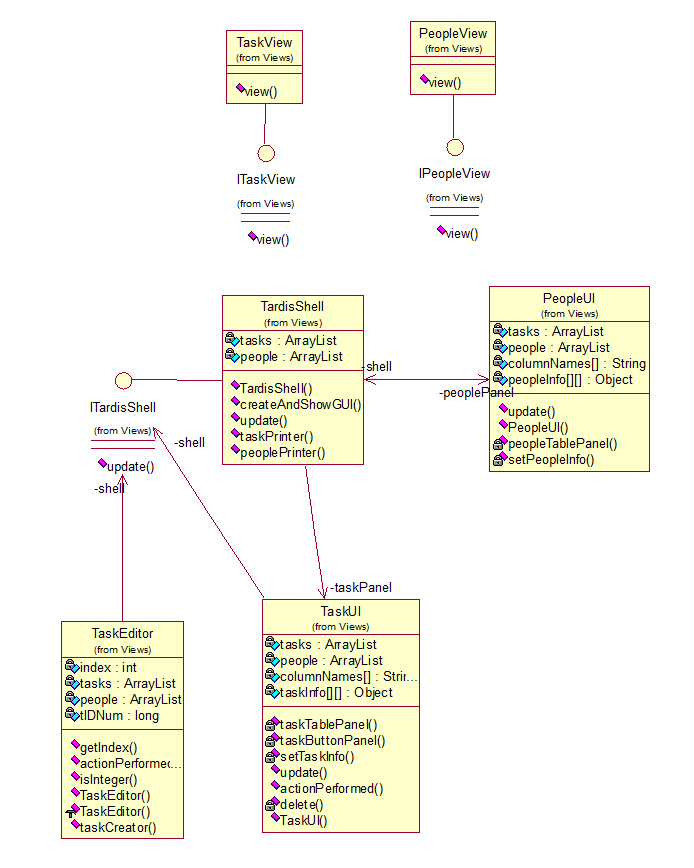
\includegraphics{subsystems/diagrams/views_class_diagram.png}

UML class diagram depicting the internal structure of the subsystem,
accompanied by a paragraph of text describing the rationale of this design.

The purpose of the views subsystem is to display the models cotained in the models subsystem. The idea was to seperate the application and presentation logic. This is used to meet the software engineering goal of loose coupling.

\subsubsection{Units Description}
\emph{PeopleUI}\\
Functions:\\
\begin{tabular}{| l | l | l | l |}
\hline
Name & Parameters & Pre-conditions & Post-conditions\\
\hline
\multirow{2}{*}{PeopleUI}{} & TardisShell shell & Requires Nothing & Ensures that\\ 
			        & ArrayList$<$Task$>$ tasks & & layout has been\\ 
                                            & ArrayList$<$Person$>$ peopleArray & &  setup.
\\
\hline
\multirow{2}{*}{peopleTablePanel} & None & Requires Nothing & Ensures that\\
& & & the table view\\
& & & for people has\\
& & & been created.
\\
\hline
\multirow{2}{*}{isCellEditable} & int rowIndex & Requires Nothing & Ensures that no cell can be\\
		 		  & int colIndex & & edited unless the edit button\\
		 		  & & &  is clicked.
\\
\hline
\multirow{2}{*}{setPeopleInfo} & None & Requires a valid list of people. & Ensures that the people data is in the table\\
		 		    & & & edited unless the edit button
\\
\hline
\multirow{2}{*}{update} & None & Requires a valid list of people. & Ensures that the people data in the table\\
		 		      & & & is up to date\\
		 		      & & &  is clicked.
\\
\hline
\end{tabular}\\
\\
Attributes:\\
\begin{tabular}{| l |}
\hline
Name\\
\hline
TardisShell shell\\
\hline
ArrayList$<$Task$>$ tasks\\
\hline
ArrayList$<$Person$>$ people\\
\hline
String[] columnNames\\
\hline
Object[][] peopleInfo\\
\hline
JPanel peopleTablePanel\\
\hline
JTable peopleTable\\
\hline
DefaultTableModel model\\
\hline
\end{tabular}

Purpose: Display the people as a table.\\
\\
\\
\emph{TaskUI}\\
Functions:\\
\begin{tabular}{| l | l | l | l |}
\hline
Name & Parameters & Pre-conditions & Post-conditions\\
\hline
\multirow{2}{*}{TaskUI}{} & ITardisShell shell & Requires Nothing & Ensures that the task\\ 
			        & ArrayList$<$Task$>$ tasks & & layout has been\\ 
                                            & ArrayList$<$Person$>$ people & & setup.
\\
\hline
\multirow{2}{*}{actionPerformed} & ActionEvent e & Requires that e            & Ensures that\\
                                                        &                        & is a valid action event. & the button press\\
                                                        &                        &                                      & was interpreted.
\\
\hline
\multirow{2}{*}{delete} & int row         & Requires that row points & Ensures that the task \\
		 	    &                     & to an existing row.          & and its subtasks\\
		 	    &                     &                                         & were deleted.\\
 			    &                     &                                         & Ensures that the task\\
                                        &                     &                                         & view was updated.
\\
\hline
\multirow{2}{*}{setTaskInfo} & None & Requires a valid list & Ensures that the task \\
		 		&          & of tasks.                   & data is in the table. 
\\
\hline
\multirow{2}{*}{update} & None & Requires a valid list & Ensures that the task data\\
		 	     &          & of tasks.                  & in the table is up to date.
\\
\hline
\multirow{2}{*}{taskButtonPanel} & None & Requires Nothing & Ensures that the add, edit\\
		 	                    &          &                             & and delete buttons have\\
                                                        &          &                             & been created.
\\
\hline
\multirow{2}{*}{taskTablePanel} & None & Requires Nothing & Ensures that the table view\\
		 	                 &           &                             & was created.
\\
\hline
\end{tabular}

Attributes:\\
\begin{tabular}{| l |}
\hline
String[] columnNames\\
\hline
DefaultTableModel model\\
\hline
ArrayList$<$Person$>$ people\\
\hline
ITardisShell shell\\
\hline
JPanel taskButtonPanel\\
\hline
Object[][] taskInfo\\
\hline
ArrayList$<$Task$>$ tasks\\
\hline
JTable taskTable\\
\hline
JPanel taskTablePanel\\
\hline
\end{tabular}\\
\\
Purpose: Display the tasks as a table.\\
\\
\\
\emph{TaskEditor}\\
Functions:\\
\begin{tabular}{| l | l | l | l |}
\hline
Name & Parameters & Pre-conditions & Post-conditions\\
\hline
\multirow{2}{*}{TaskEditor} & ITardisShell shell                         & Requires Nothing & Ensures that the task\\ 
			          & ArrayList$<$Task$>$ tasks       &                             & editor has been created.\\ 
                                              & ArrayList$<$Person$>$ people &                             & 
\\
\hline
\multirow{2}{*}{TaskEditor} & ITardisShell shell                         & Requires Nothing & Ensures that the task\\ 
			          & ArrayList$<$Task$>$ tasks       &                             & editor has been created\\ 
                                              & ArrayList$<$Person$>$ people &                             & and populated with the data\\
			          & int index                                      &                             & of the selected element.
\\
\hline
\multirow{2}{*}{actionPerformed} & ActionEvent e & Requires that e            & Ensures that\\
                                                        &                        & is a valid action event. & the button press\\
                                                        &                        &                                      & was interpreted.
\\
\hline
\multirow{2}{*}{int getIndex} & None & Requires Nothing & Ensures that the index.\\
		                         &           &                             & is returned.
\\
\hline
\multirow{2}{*}{bool isInteger} & String in & Requires Nothing & Ensures that the question,\\
		 	                &               &                             & is the string an integer\\
		 	                &               &                             & is answered.
\\
\hline
\multirow{2}{*}{taskCreator} & long taskId                    & Requires Nothing & Ensures that either a new task\\
		 	             & String title                     &                             & was created or an existing\\
                                                 & String shortDescription &                             & task was modified.\\
				 & int duration                   &                             & \\
				 & String deliverable          &                             &\\
		       		 & Date dueDate               &                             &\\
				 & int personID                  &                             &\\
				 & Task parent                   &                             &
\\
\hline
\end{tabular}

Attributes:\\
\begin{tabular}{| l |}
\hline
JButton CANCEL\\
\hline
JComboBox cPeople\\
\hline
JComboBox cSuper\\
\hline
JLabel cSuperL\\
\hline
JLabel deliverable\\
\hline
JLabel dueDateD\\
\hline
JLabel dueDateM\\
\hline
JLabel dueDateY\\
\hline
JLabel duration\\
\hline
int index\\
\hline
JPanel panel\\
\hline
ArrayList$<$Person$>$ people\\
\hline
JLabel personID\\
\hline
ITardisShell shell\\
\hline
JLabel shortDesc\\
\hline
JButton SUBMIT\\
\hline
JLabel superID\\
\hline
JLabel taskID\\
\hline
ArrayList$<$Task$>$ tasks\\
\hline
TextField tDay\\
\hline
TextField tDeliverable\\
\hline
TextField tDesc\\
\hline
TextField tDuration\\
\hline
JLabel tID\\
\hline
long tIDNum\\
\hline
JLabel title\\
\hline
TextField tMonth\\
\hline
TextField tTitle\\
\hline
TextField tYear\\
\hline
\end{tabular}\\
\\
Purpose: Add and edit a task.\\
\\
\\
List each class in this subsystem and write a short description of its purpose,
as well as notes or reminders useful for the programmers who will implement them.
List all attributes and functions of the class.